\section{Handson}

\begin{frame}
	\frametitle{Hands-on PTracking}
	\framesubtitle{Getting the library}
	
	\emph{PTracking} is currently available in the following private GitHub repository:
	\begin{center}
		\url{https://github.com/fabioprev/ptracking}
	\end{center}
	
	A request for getting access is required:
	\begin{center}
		\url{previtali@dis.uniroma1.it}
	\end{center}
	
	Currently the only supported development platform is \textbf{Linux}.
\end{frame}

\begin{frame}
	\frametitle{Hands-on PTracking}
	\framesubtitle{Dependencies}
	
	On Xubuntu (Ubuntu) 14.04 LTS (kernel 3.13.0-37) and later versions, you need to install
	the following packages
	
	\vspace{0.2cm}
	
	\begin{columns}[T]
		\column{.5\textwidth}
		
		\begin{itemize}
			\item build-essential
			\item cmake
			\item libxml2
			\item libxml2-dev
			\item libboost1.54-all-dev
		\end{itemize}
		
		\column{.5\textwidth}
		\centering
		
		\begin{itemize}
			\item libcgal-dev
			\item libopencv-dev
			\item libopenni2-dev (optional)
			\item gnuplot (optional)
			\item gnuplot-x11 (optional)
		\end{itemize}
	\end{columns}
\end{frame}

\begin{frame}
	\frametitle{Hands-on PTracking}
	\framesubtitle{Building the library}
	
	We recommend a so-called out of source build which can be achieved by the following command
	sequence
	
	\vspace{0.2cm}
	
	\begin{itemize}
		\item \texttt{cd <PTracking-root-directory>}
		\item \texttt{mkdir build}
		\item \texttt{cd build}
		\item \texttt{cmake ../src}
		\item \texttt{make -j<number-of-cores+1>}
	\end{itemize}
\end{frame}

\begin{frame}
	\frametitle{Hands-on PTracking}
	\framesubtitle{Installing the library}
	
	\vspace{0.4cm}
	
	The library can be optionally installed by typing the following command sequence
	
	\vspace{0.2cm}
	
	\begin{itemize}
		\item \texttt{cd <PTracking-root-directory>/build}
		\item \texttt{sudo make install}
	\end{itemize}
	
	\vspace{0.15cm}
	
	\textbf{Header files:} \texttt{/usr/local/include/PTracking} \\
	
	\vspace{0.15cm}
	
	\textbf{Shared objects:} \texttt{/usr/local/lib/PTracking} \\
	
	\vspace{0.15cm}
	
	\textbf{Binaries:} \texttt{/usr/local/bin} \\
	
	\vspace{0.75cm}
	
	\textbf{Warning:} You first need to logout before starting using the library, because the
	\texttt{$ \sim $/.profile} file has been modified
\end{frame}

\begin{frame}
	\frametitle{Project}
	
	\vspace{0.5cm}
	
	\setstretch{1}
	To whom is interested in doing a project about multiple object tracking using heterogeneous
	sensors, just need to drop me an email at \url{previtali@dis.uniroma1.it}\\
	
	\vspace{-0.3cm}
	
	\begin{center}
		\begin{tikzpicture}
			\node at (0,0) [draw=white,ultra thick,inner sep=0pt]
			{
				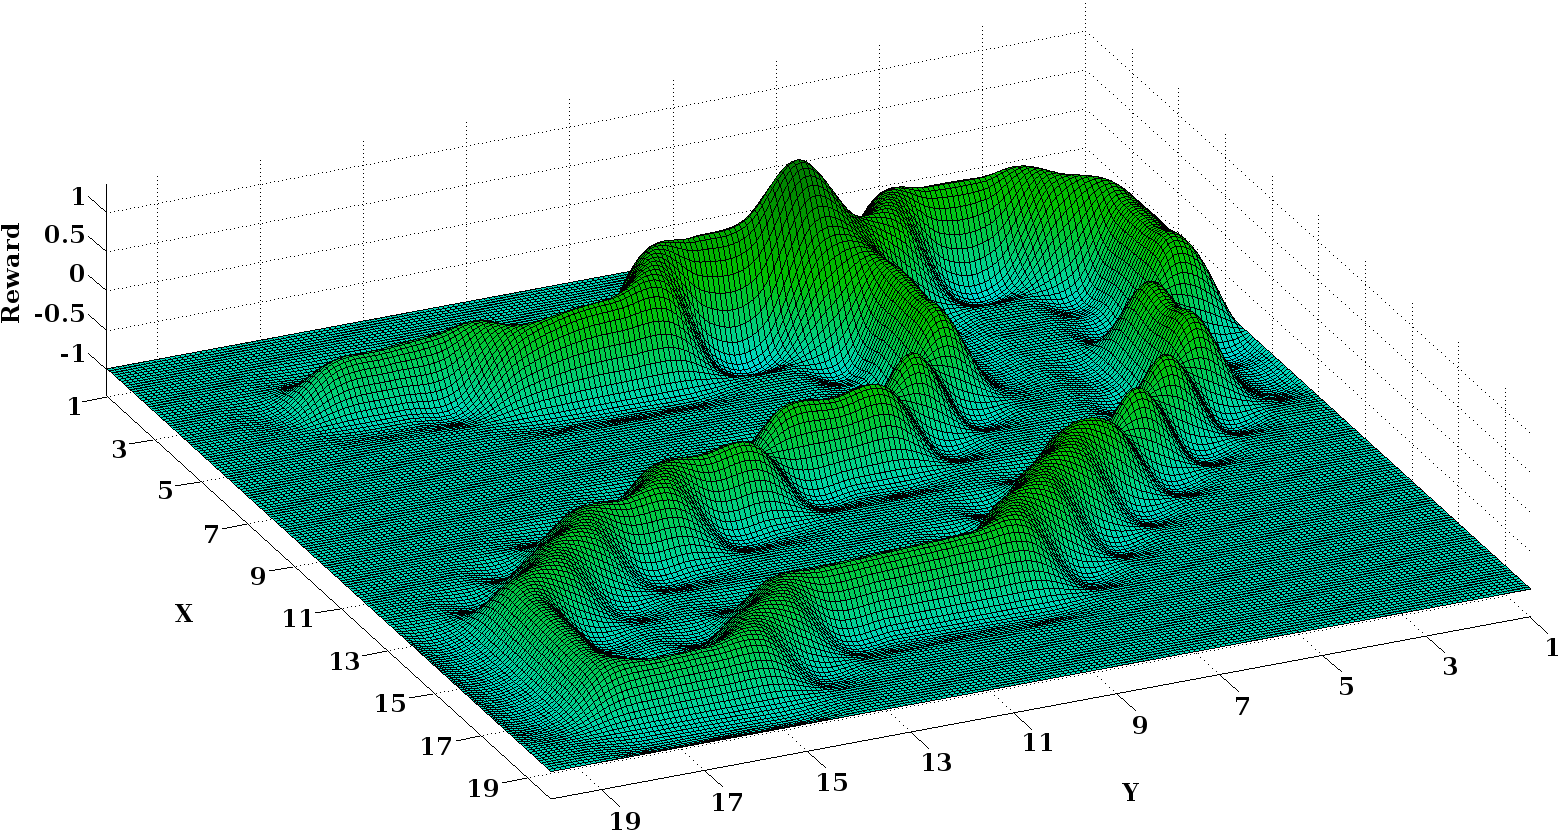
\includegraphics[scale=0.23]{Figures/IRL-Model.png}
			};
		\end{tikzpicture}
	\end{center}
\end{frame}
